\chapter{Wdrożenie i testowanie aplikacji}

W tej części zostały zamieszczone obrazy działania wprowadzonej aplikacji. Aplikacja działa
poprawnie i zgodnie z przewidywaniami. \\

Na rysunkach od \ref{fig:addFilm} do \ref{fig:endAddFilm} zademonstrowane zostało działanie replikacji na przykładzie dodawania filmu do bazy z poziomu aplikacji webowej.\\

Na rysunku \ref{fig:addFilm} wpisane zostały dane przykładowego filmu, a po naciśnięciu przycisku 'Dodaj film' aplikacja poprzez API REST łączy się z węzłem master rozproszonej bazy danych, gdyż wprowadzana będzie modyfikacja, a następnie dodaje dane do tabeli Filmy (rysunek \ref{fig:FilmMaster}) dzięki procedurze SQL 'DodajFilm'. Wykonana procedura zostaje replikowana do wszystkich węzłów Slave. Tabela Filmy dla wybranego węzła Slave na porcie 8083 została pokazana na rysunku \ref{fig:FilmSlave}. Z węzła Slave również odczytywane są dane poprzez aplikację kliencką, a poprawnie odczytane dane z takiego węzła zostały przedstawione na rysunku \ref{fig:endAddFilm}.

\begin{figure} [H]
	\centering
	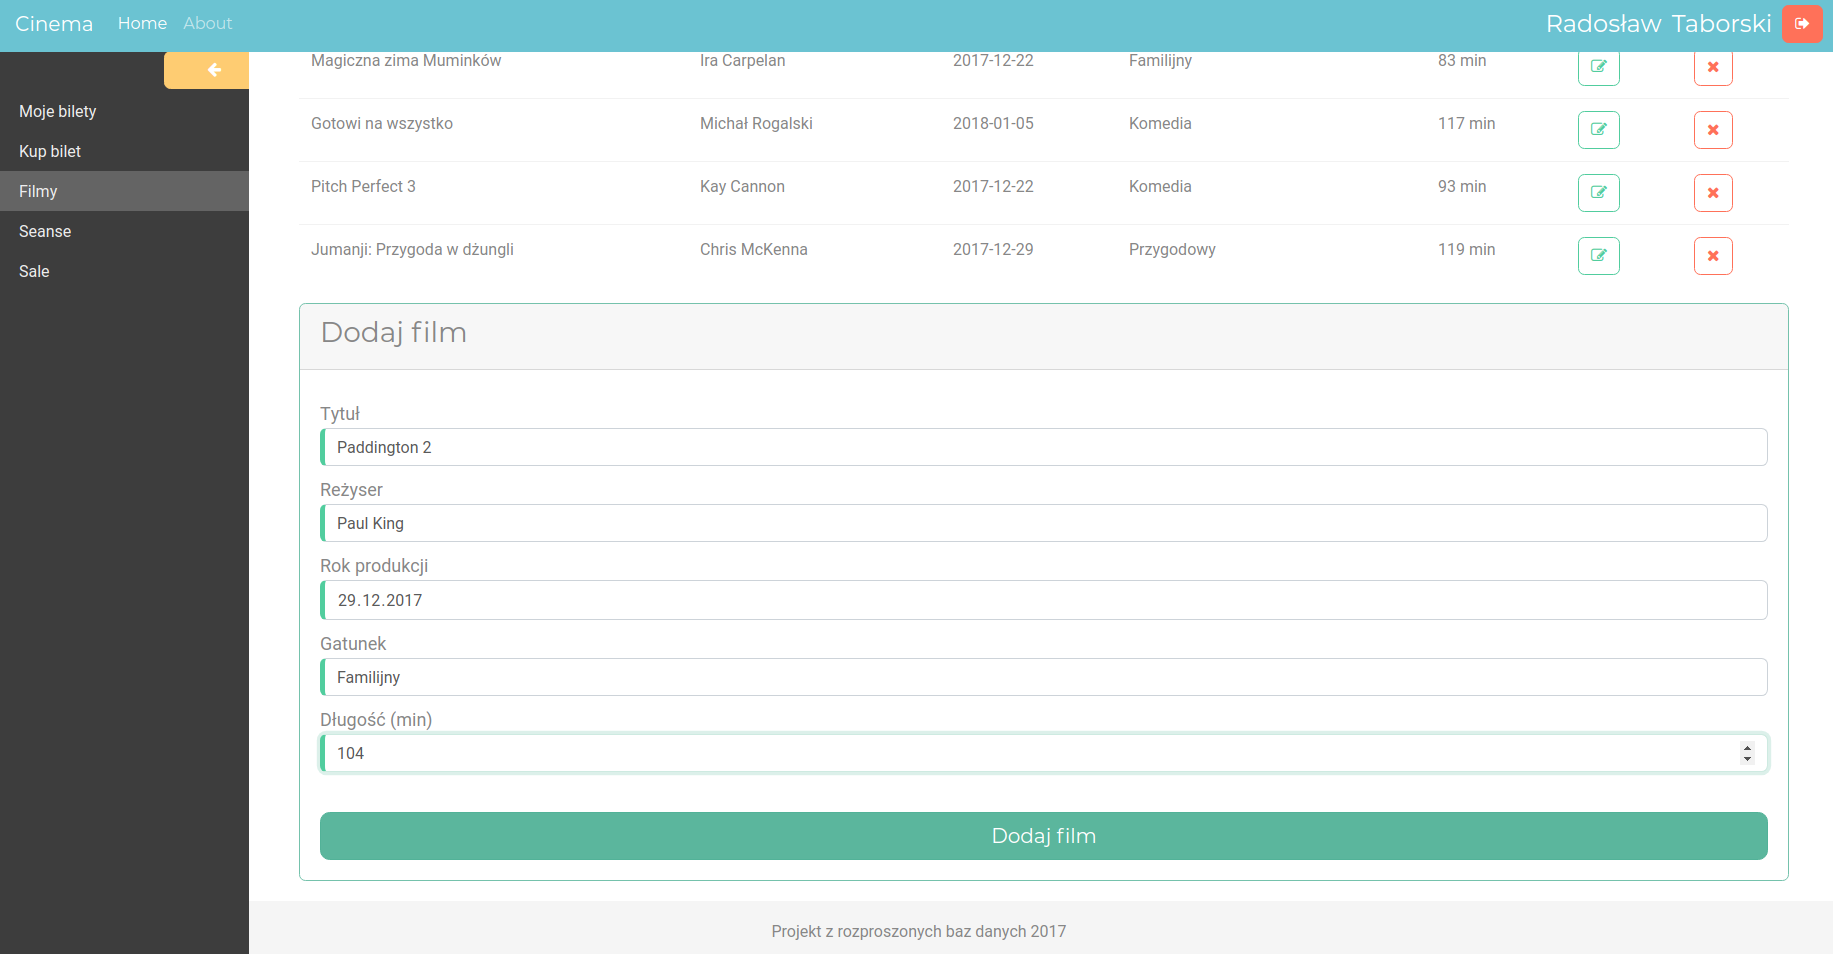
\includegraphics[width=1\linewidth]{rozdzial06/5.png}
	\caption{Dodawanie nowego filmu poprzez aplikację}
	\label{fig:addFilm}
\end{figure}

\begin{figure} [H]
	\centering
	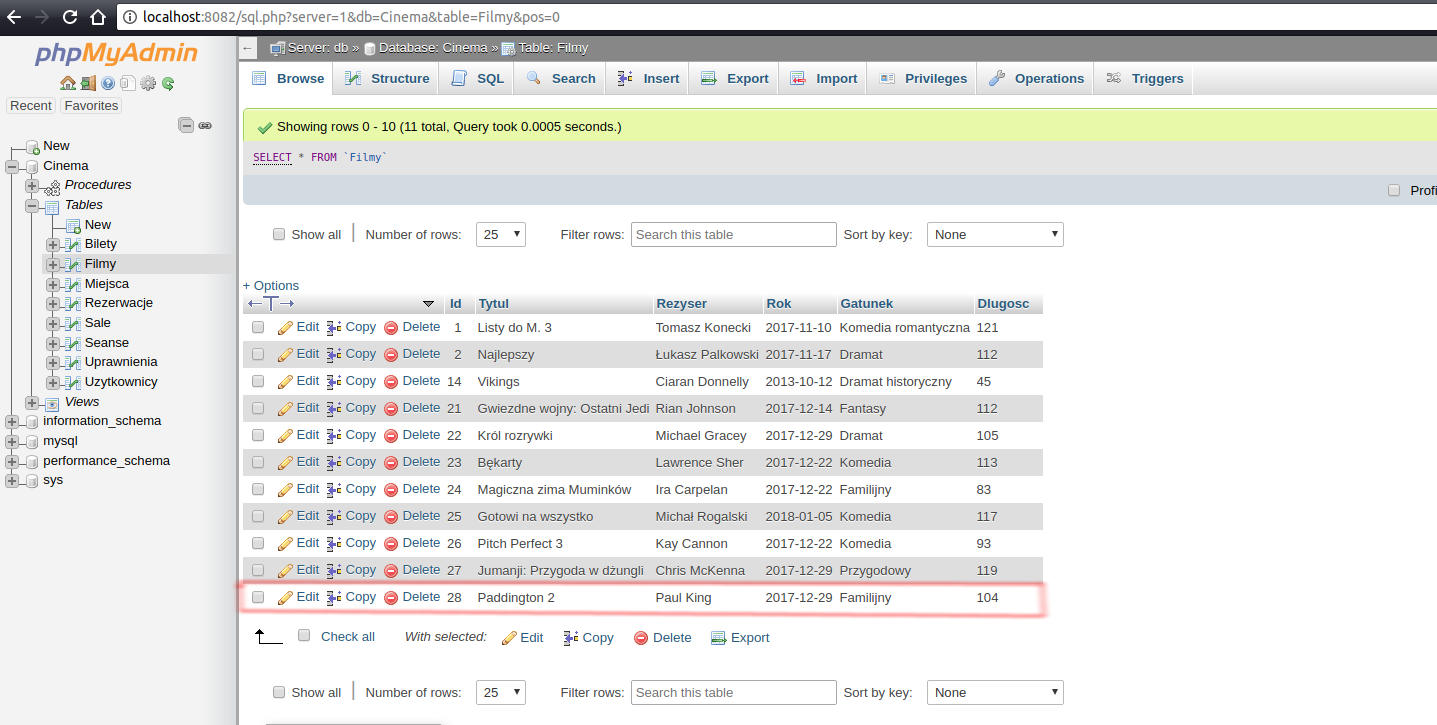
\includegraphics[width=1\linewidth]{rozdzial06/7.png}
	\caption{Tabela Filmy na węźle \textit{master} o porcie 8082}
	\label{fig:FilmMaster}
\end{figure}

\begin{figure} [H]
	\centering
	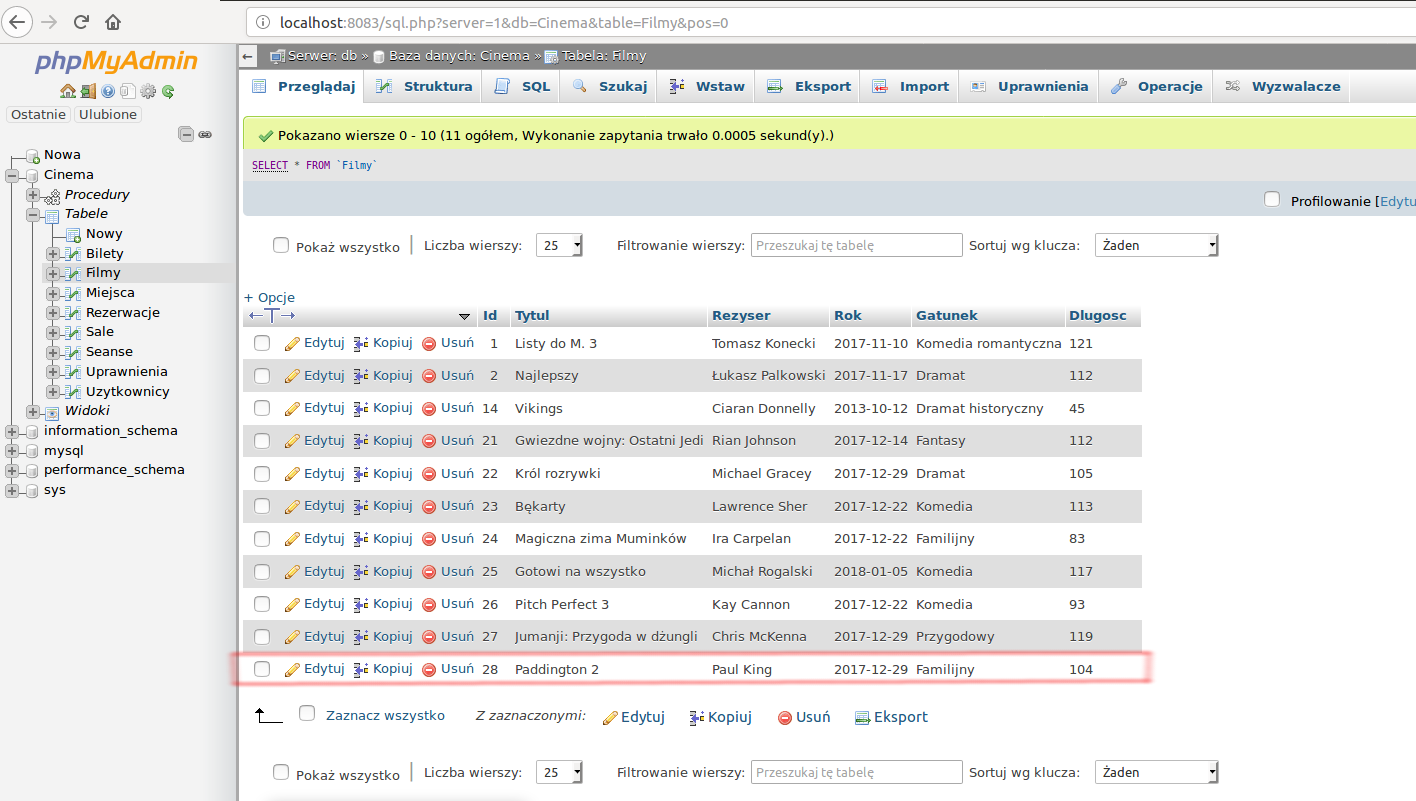
\includegraphics[width=1\linewidth]{rozdzial06/8.png}
	\caption{Tabela Filmy na węźle \textit{slave} 1 o porcie 8083}
	\label{fig:FilmSlave}
\end{figure}

\begin{figure} [H]
	\centering
	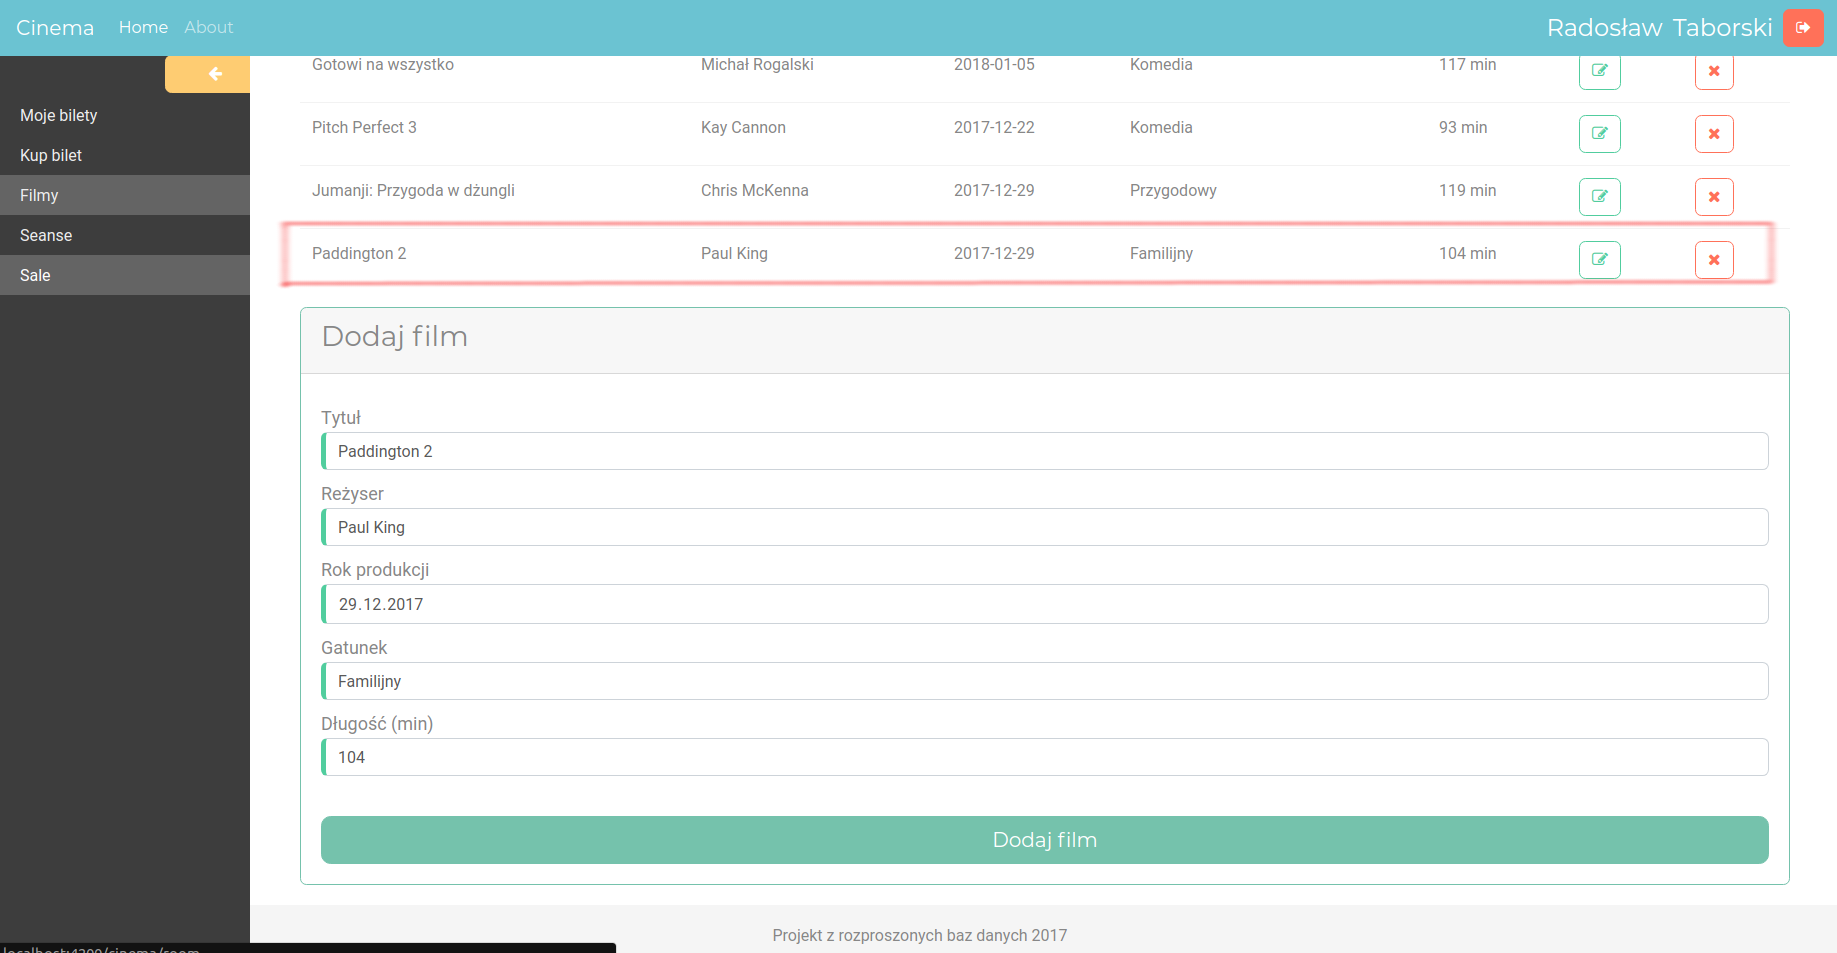
\includegraphics[width=1\linewidth]{rozdzial06/6.png}
	\caption{Nowy film wyświetlany w aplikacji}
	\label{fig:endAddFilm}
\end{figure}

Tak jak to już zostało wspomniane w podrozdziale \ref{chap:testReplikacji}, by replikacja mogła przebiegać prawidłowo, bazy na węzłach \textit{slave} muszą być spójne z bazą na węźle \textit{master}, a co z tego poniekąd wynika bazy na wezłach \textit{slave} muszą być utworzone i muszą posiadać taką samą strukturę tabel.

